\documentclass[12pt,a4paper]{article}

% Package to include code
\usepackage{michel}
\usepackage{listings}
\usepackage{inconsolata}
\usepackage{color}
\usepackage{varioref}

\usepackage{tikz}
\usetikzlibrary{trees}
\usepackage{pgfplots}
\lstset{language=Python}
\lstset{numbers=none, basicstyle=\ttfamily\footnotesize,
  numberstyle=\tiny,keywordstyle=\color{blue},stringstyle=\ttfamily,showstringspaces=false}
\lstset{backgroundcolor=\color[rgb]{0.95 0.95 0.95}}
\lstdefinestyle{numbers}{numbers=left, stepnumber=1,
  numberstyle=\tiny,basicstyle=\footnotesize, numbersep=10pt}
\lstdefinestyle{nonumbers}{numbers=none}
\lstset{
  breaklines=true,
  breakatwhitespace=true,
}

\newcommand*{\examplesPath}{../../examples}

% Font selection: uncomment the next line to use the ``beton'' font
%\usepackage{beton}

% Font selection: uncomment the next line to use the ``times'' font
%\usepackage{times}

% Font for equations
\usepackage{euler}


%Package to define the headers and footers of the pages
\usepackage{fancyhdr}


\title{
  \vspace{-3cm}
  \epsfig{figure=transp-or.eps,height=2cm}
  \hfill
  \epsfig{figure=epfl,height=1.5cm}   \\*[-0.5cm]
  \mbox{}\hrulefill\mbox{} \\*[3cm] Arithmetic expressions in Biogeme}

\author{Michel Bierlaire}
\date{August 5, 2024}


\begin{document}


\begin{titlepage}
  \pagestyle{empty}

  \maketitle
  \vspace{2cm}

  \begin{center}
    \small Report TRANSP-OR 240805 \\ Transport and Mobility Laboratory \\ School of Architecture, Civil and Environmental Engineering \\ Ecole Polytechnique F\'ed\'erale de Lausanne \\ \verb+transp-or.epfl.ch+
    \begin{center}
      \textsc{Series on Biogeme}
    \end{center}
  \end{center}


  \clearpage
\end{titlepage}


The package Biogeme (\texttt{biogeme.epfl.ch}) is designed to estimate
the parameters of various models using maximum likelihood
estimation. It is particularly designed for discrete choice
models.

This document describes how Biogeme handles arithmetic expressions and
deals with potential numerical issues. The concepts have been
implemented in  \lstinline+cythonbiogeme 1.0.4+, used by
\lstinline+biogeme 3.2.14+.


\section{Introduction}\label{eq:intro}

The core of the Biogeme software package is the calculation of
formulas for each observation in a database. In estimation mode, the
formula is the log likelihood function. And its derivatives are
necessary for the optimization algorithm as well as the calculation of
useful statistics.  In simulation mode, the formulas are any indicator
that the analyst deems useful to calculate (choice probabilities,
elasticities, etc.) We refer the reader to \citeasnoun{Bier18a} and
\citeasnoun{Bier23} for more details about the use of Biogeme for
model estimation and the calculation of indicators.


To allow the user to use Biogeme on a wide variety of model
specifications, the formulas are composed of elementary arithmetic
operations. These building blocks are organized in a complex tree structure, where each of them receives inputs from others, generates output, that is forwarded to the next layer.
For instance, the formula
\[
-x + \frac{\exp(y - 1)}{2}
\]
can be represented as illustrated in Figure~\ref{fig:tree}.

\begin{figure}[htb]
  \begin{center}
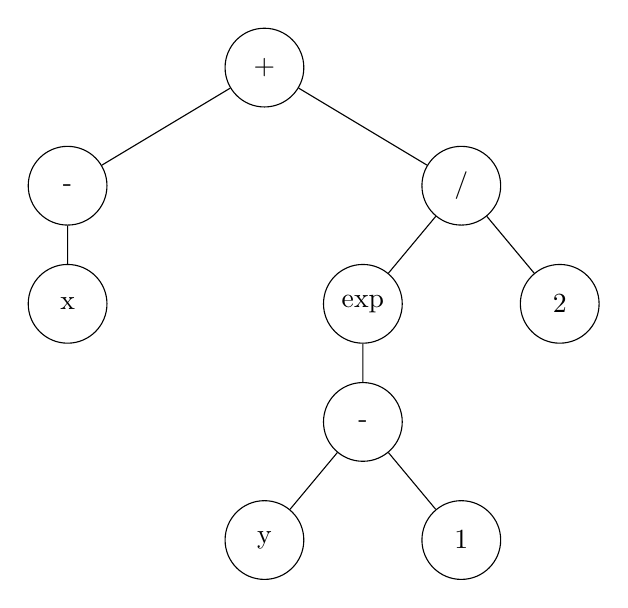
\begin{tikzpicture}[level distance=1.5cm,
  level 1/.style={sibling distance=5cm},
  level 2/.style={sibling distance=2.5cm},
  every node/.style={circle, draw, minimum size=1cm, inner sep=0pt, align=center}
  ]
  \node {+}
    child {
      node {-} 
      child {node {x}}
    }
    child {
      node {/}
      child {
        node {exp}
        child {
          node {-}
          child {node {y}}
          child {node {1}}
        }
      }
      child {node {2}}
    };
\end{tikzpicture}
  \end{center}
\caption{\label{fig:tree}Tree representation of a formula}
\end{figure}

Each node of the formula is associated with a specific simple
operation, and is in charge of calculating its value, and its
derivatives.


Computers are working with finite arithmetic. It means that computers
have limitations in the way they represent and operate on numbers due
to their finite hardware resources and the design of numerical
representations.  Therefore, the actual implementation of the
arithmetic operations are not necessarily an exact duplicate of their
mathematical equivalent, that considers a continuous space of real
numbers, that can take any value.

The objective of this document is to describe how each arithmetic expression is handled by Biogeme.
Note that, by default, Biogeme follows the IEEE standard (\cite{IEEE:2019aa}) that specify formats and operations for floating-point arithmetic, including the definition of exception conditions
and the handling of these conditions. For instance,  the calculation of $\ln(0)$  results in
$-\infty$, and the calculation of $\ln(-1)$ results in NaN (Not a Number). Those standards are not reviewed in this document.

\section{Numerical limits}

The computer representation of a real number is called a ``floating-point'' representation. It is divided into three parts. The values of the parameters below correspond to a 64-bit representation:
\begin{itemize}
\item A sign bit $s$, that indicates the sign of the number (0 for positive, 1 for negative).
\item An exponent $e$ covering $k=11$ bits, that represents the exponent of the number in a biased form. By bias, it is meant that negative and positive powers of two are possible. The bias $b$ is added to obtain a positive number. The bias is $b=2^{k-1}-1=1023$, so that the exponents range between -1022 to +1023.
\item A mantissa ($m$), using $p-1$ bits, where $p$ is the precision. 
\end{itemize}
So, for a 64-bit representation, $s+k+p-1=64$, so that $p=53$.
Therefore, the value of a floating point number is
\[
(-1)^s (1+m) 2^{e-b}.
\]

This representation allows for only a finite quantity of real numbers to be represented: $2^{64} \approx 10^{19}$ numbers. And this imposes numerical limits. In Python, it is possible to retrieve information about those limits using \lstinline+numpy+. If you type \lstinline+print(np.finfo(float))+, you obtain:
\begin{lstlisting}
Machine parameters for float64
---------------------------------------------------------------
precision =  15   resolution = 1.0000000000000001e-15
machep =    -52   eps =        2.2204460492503131e-16
negep =     -53   epsneg =     1.1102230246251565e-16
minexp =  -1022   tiny =       2.2250738585072014e-308
maxexp =   1024   max =        1.7976931348623157e+308
Nexp =       11   min =        -max
smallest_normal = 2.2250738585072014e-308   smallest_subnormal = 4.9406564584124654e-324
---------------------------------------------------------------  
\end{lstlisting}



In this document, we consider $\varepsilon$, the ``machine epsilon'', that is the difference between 1.0 and the next smallest representable float larger than 1.0. It is an important value, because it means that, for each $x < \varepsilon$, adding $x$ to 1 will provide 1 as a result:
\[
1 + x = 1.
\]
This may clearly lead to unpredictable behavior of numerical calculations. As mentioned in the output of \lstinline+numpy+, the value of the machine epsilon in 64-bit representation is
\[
\varepsilon \approx 10^{-16}.
\]
There is an empirical way to calculate this value, using the following script:
\begin{lstlisting}
epsilon = 1
while 1.0 + epsilon != 1.0:
    epsilon /= 2.0
epsilon *= 2.0
\end{lstlisting}

In Biogeme, we consider 
  \[
  \xi = \sqrt{\varepsilon}
  \]
to determine if a value is sufficiently close to zero.  Specifically,
Biogeme applies special handling to any value $x$ such that $-\xi
\leq x \leq 0$. For instance, $\ln(-10^{-10})$ is treated as $\ln(0)=-\infty$ in Biogeme, whereas  the IEEE standard would produce NaN.
es
\section{Expressions}

We explicitly characterize how each
arithmetic expression is implemented in Biogeme. Each expression in
Biogeme is represented by an object of generic type
\lstinline+Expression+.



The document is organized by groups of expressions:
\begin{itemize}
\item Elementary expressions, including the numbers, the variables, the parameters, etc.
\item The unary expressions, accepting one input value.
\item The comparison expressions, accepting two input values, and used to compare two expressions.
\item Other binary expressions, accepting two input values.
\item The n-ary expressions, accepting more than two values.
\item The logit expression, implementing the logit model.
\end{itemize}



\subsection{Elementary expressions}

The elementary expressions are the building blocks of any expression. They correspond to the leaves of the tree representation, such as the one illustrated in Figure~\ref{fig:tree}.  

\begin{description}
\item[Numeric values] Numeric values are the most basic expressions. The syntax for numeric values is
  \begin{lstlisting}
    Numeric(x)
  \end{lstlisting}
  where \lstinline+x+ is the value. In most cases, the user does not need to use this syntax, as Biogeme tries to identify them automatically.
\item[Variables] Variables are referring to the columns of the data set:
  \begin{lstlisting}
    Variable('name_of_the_variable')
  \end{lstlisting}
  This expression simply returns the value of the corresponding variable for the current row. 
\item[Random variable] A random variable is used in the context of numerical integration.
  The syntax is
  \begin{lstlisting}
    RandomVariable('name_of_the_random_variable').
  \end{lstlisting}
\item[Draws] Random draws are used in the context of Monte-Carlo integration. 
  The syntax is
  \begin{lstlisting}
    bioDraws('name_of_the_draws', draw_type)
  \end{lstlisting}
  where \lstinline+draw_type+ is a string. It can refer to  a user defined type of draws, or one of the native draws from the following list:
  \begin{lstlisting}
'UNIFORM', 'UNIFORM_ANTI', 'UNIFORM_HALTON2', 'UNIFORM_HALTON3', 'UNIFORM_HALTON5', 'UNIFORM_MLHS', 'UNIFORM_MLHS_ANTI', 'UNIFORMSYM', 'UNIFORMSYM_ANTI', 'UNIFORMSYM_HALTON2', 'UNIFORMSYM_HALTON3', 'UNIFORMSYM_HALTON5', 'UNIFORMSYM_MLHS', 'UNIFORMSYM_MLHS_ANTI', 'NORMAL', 'NORMAL_ANTI', 'NORMAL_HALTON2', 'NORMAL_HALTON3', 'NORMAL_HALTON5', 'NORMAL_MLHS', 'NORMAL_MLHS_ANTI'
  \end{lstlisting}
\item[Parameters] Parameters must be estimated from data. Their first values is defined by the user. There are two categories of parameters. Free parameters are updated by the optimization algorithm.
  Fixed parameters are not.
  The syntax for parameters is
  \begin{lstlisting}
    Beta('name_of_the_parameter', x_0, ell, u, fixed)
  \end{lstlisting}
  where \lstinline+x_0+ is the initial value of the parameter,
  \lstinline+ell+ is the lower bound on the parameter, \lstinline+u+ is the upper bound on the parameter, and \lstinline+fixed+ specifies if the parameter must be fixed (\lstinline+fixed=1+) of free (\lstinline+fixed=0+).
\end{description}

Biogeme calculates derivatives with respects to the \lstinline+Beta+ parameters. In the following, we denote by $\beta_i$ and $\beta_j$ the literals that are involved in the derivatives.
Obviously, we have
\[
\frac{\partial \beta_i}{\partial \beta_i}=1, \;
\frac{\partial \beta_i}{\partial \beta_j}=0, \;
\]
and
\[
\frac{\partial^2 \beta_i}{\partial \beta_i^2}=\frac{\partial^2 \beta_i}{\partial \beta_i \partial \beta_j} = 0. 
\]


\subsection{Unary expressions}

Unary expressions take one value as input. Like any expression, they return a value and the derivatives.
\begin{description}
\item[Unary minus]
  Syntax: if \lstinline+y+ is the input value, the unary minus is
  \begin{lstlisting}
    -y
  \end{lstlisting}
  If $y$ is the input value, it returns $f(y)=-y$. 
  The derivatives are:
  \[
  \frac{\partial f}{\partial \beta_i} = - \frac{\partial y}{\partial \beta_i}
  \]
  and
  \[
  \frac{\partial^2 f}{\partial \beta_i \partial \beta_j} = - \frac{\partial y}{\partial \beta_i \partial \beta_j}.
  \]
\item[Exponential] If \lstinline+y+ is the input value, the syntax is
  \begin{lstlisting}
    exp(y)
  \end{lstlisting}
  Let $y$ be the input value.
  \begin{align*}
    f(y)&= e^y, \\
    \frac{\partial f(y)}{\partial \beta_i} &= e^y \frac{\partial y}{\partial \beta_i}, \\
    \frac{\partial^2 f(y)}{\partial \beta_i \partial \beta_j} &= e^y \frac{\partial y}{\partial \beta_i}\frac{\partial y}{\partial \beta_j} + \frac{\partial^2 y}{\partial \beta_i \partial \beta_j}.
  \end{align*}

\item[Logarithm] If \lstinline+y+ is the input value, the syntax is
  \begin{lstlisting}
    log(y)
  \end{lstlisting}
  
  Biogeme considers a negative $y$ that is close to zero to be 0:
  \[
  y \leftarrow 0, \text{ if } y < 0 \text{ and } y \geq -\xi.
  \]
  Let $y$ be the input value, processed as described above.
    \begin{align*}
    f(y)& =\ln(y), \\ 
    \frac{\partial f(y)}{\partial \beta_i} &= \frac{1}{y} \frac{\partial y}{\partial \beta_i}, \\
    \frac{\partial^2 f(y)}{\partial \beta_i \partial \beta_j} &=
    -\frac{1}{y^{2}}
    \frac{\partial y}{\partial \beta_i}
    \frac{\partial y}{\partial \beta_j }
    + \frac{1}{y}
    \frac{\partial^2 y}{\partial \beta_i \partial \beta_j}.
    \end{align*}


\item[Logarithm or zero] This expression is the same as the logarithm,
  except that if the argument is exactly zero, it returns 0. For any
  value different from zero, it returns the same as for the log
  expression. It is designed as a shortcut for the expression
  \begin{lstlisting}
    Elem({1: 0, 0: log(x)}, x == 0).
  \end{lstlisting}

  If \lstinline+y+ is the input value, the syntax is
  \begin{lstlisting}
    logzero(y)
  \end{lstlisting}
  Biogeme considers a negative $y$ that is close to zero to be 0:
  \[
  y \leftarrow 0, \text{ if } y < 0 \text{ and } y \geq -\xi.
  \]
  Let $y$ be the input value, processed as described above.
    \begin{align*}
      f(y) &=  0,\\
      \frac{\partial f(y)}{\partial \beta_i} &= 0,\\
      \frac{\partial^2 f(y)}{\partial \beta_i\partial \beta_j} &= 0.\\
    \end{align*}
  \item If $y > 0$, we define
    \begin{align*}
    f(y)& =\ln(y), \\ 
    \frac{\partial f(y)}{\partial \beta_i} &= \frac{1}{y} \frac{\partial y}{\partial \beta_i}, \\
    \frac{\partial^2 f(y)}{\partial \beta_i \partial \beta_j} &=
    -\frac{1}{y^{2}}
    \frac{\partial y}{\partial \beta_i}
    \frac{\partial y}{\partial \beta_j }
    + \frac{1}{y}
    \frac{\partial^2 y}{\partial \beta_i \partial \beta_j}.
    \end{align*}



 \item[Sinus] If \lstinline+y+ is the input value, the syntax is
  \begin{lstlisting}
    sin(y)
  \end{lstlisting}
  Let $y$ be the input value. We define
  \begin{align*}
      f(y) &= \sin(y), \\
      \frac{\partial f(y)}{\partial \beta_i} &= \cos(y) \frac{\partial y}{\partial \beta_i},\\
      \frac{\partial^2 f(y)}{\partial \beta_i\partial \beta_j} &= -\sin(y)\frac{\partial y}{\partial \beta_i}\frac{\partial y}{\partial \beta_j} + \cos(y)\frac{\partial^2 y}{\partial \beta_i\partial \beta_j}.\\
  \end{align*}

 \item[Cosinus] If \lstinline+y+ is the input value, the syntax is
  \begin{lstlisting}
    cos(y)
  \end{lstlisting}
  Let $y$ be the input value. We define
  \begin{align*}
      f(y) &= \cos(y), \\
      \frac{\partial f(y)}{\partial \beta_i} &= -\sin(y) \frac{\partial y}{\partial \beta_i},\\
      \frac{\partial^2 f(y)}{\partial \beta_i\partial \beta_j} &= -\cos(y) \frac{\partial y}{\partial \beta_i} \frac{\partial y}{\partial \beta_j}- \sin(y)\frac{\partial^2 y}{\partial \beta_i\partial \beta_j}.\\
  \end{align*}
    
\item[Derive] This expression calculates the derivative of the input
  with respect to one of the literals. If \lstinline+y+ is the
  input expression, the syntax for its derivative with respect to a
  literal \lstinline+beta+ is
  \begin{lstlisting}
    Derive(y, 'beta')
  \end{lstlisting}
  Let $y$ be the input value. Then,
  \[
  f(y) = \frac{\partial y}{\partial \beta}.
  \]
  The derivatives of this expression are not evaluated by Biogeme. It is meant to be used in simulation mode only.

\item[Integrate] This expression performs numerical integration
of Biogeme expressions using the Gauss-Hermite quadrature method. The integration is performed over a random variable, and the method can compute both gradients and hessians of the integrated function.

If takes as argument an expression
  \lstinline+y+ that includes a random variable
  \lstinline+omega+. The syntax is
  \begin{lstlisting}
    Integrate(y, 'omega')
  \end{lstlisting}
  Let $y$ be the input value. We define
  \begin{align*}
    f(y) &= \int_{-\infty}^{+\infty} y(\omega) d\omega, \\
    \frac{\partial f(y)}{\partial \beta_i} &= \int_{-\infty}^{+\infty} \frac{\partial y(\omega)}{\partial \beta_i} d\omega,\\
    \frac{\partial^2 f(y)}{\partial \beta_i\partial \beta_j} &=  \int_{-\infty}^{+\infty} \frac{\partial^2 y(\omega)}{\partial \beta_i \partial \beta_j} d\omega.\\
  \end{align*}

  
\item[MonteCarlo] This expression approximates an integral using Monte-Carlo integration.
If takes as argument an expression
  \lstinline+y+ that includes draws.
The syntax is
  \begin{lstlisting}
    MonteCarlo(y)
  \end{lstlisting}
  Let $y$ be the input value. We define
  \begin{align*}
    f(y) &= \frac{1}{R}\sum_{r=1}^R y(\xi_r), \\
    \frac{\partial f(y)}{\partial \beta_i} &= \frac{1}{R}\sum_{r=1}^R \frac{\partial y(\xi_r)}{\partial \beta_i}, \\
    \frac{\partial^2 f(y)}{\partial \beta_i\partial \beta_j} &= \frac{1}{R}\sum_{r=1}^R \frac{\partial^2 y(\xi_r)}{\partial \beta_i \partial \beta_j}, \\
  \end{align*}
  where $R$ is a parameter defining the number of draws to be used, and $\xi_r$ are the values of the draws.
  
\item[bioNormalCdf] This expression provides an analytical approximation of the cumulative distribution function of a normal random variable. If \lstinline+y+ is the input, the syntax is
  \begin{lstlisting}
    bioNormalCdf(y).
  \end{lstlisting}
The routine calculates the CDF of the normal distribution, $\Phi(y)$, for a given input expression $y$, along with its gradient and hessian. The CDF of the normal distribution is defined as:
\[
\Phi(y) = \frac{1}{2} \left[ 1 + \frac{2}{\sqrt{\pi}} \int_0^{\frac{y}{\sqrt{2}}} e^{-t^2} \, dt \right]
\]

To approximate the normal CDF, the method relies on numerical
techniques involving series expansions and the incomplete gamma
function.

The probability density function (pdf) of the normal distribution, $\phi(y)$, is given by:
\[
\phi(y) = \frac{1}{\sqrt{2\pi}} \exp\left( -\frac{y^2}{2} \right).
\]

The gradient of the CDF with respect to the input variables is calculated as:
\[
\frac{\partial \Phi(y)}{\partial \beta_i} = \phi(y) \frac{\partial y}{\partial \beta_i}
\]
where $\frac{\partial y}{\partial \beta_i}$ are the partial derivatives of the input expression $y$.

The hessian matrix of the CDF is computed as:
\[
\frac{\partial^2 \Phi(y)}{\partial \beta_i \partial \beta_j} = \phi(y) \frac{\partial^2 y}{\partial \beta_i \partial \beta_j} - \phi(y) y \frac{\partial y}{\partial \beta_i} \frac{\partial y}{\partial \beta_j}
\]
where $\frac{\partial^2 y}{\partial \beta_i \partial \beta_j}$ are the second-order partial derivatives of the input expression $y$.


\item[Belongs to] This expression verifies if the input value belongs to a set. 
If \lstinline+y+ is the input, the syntax is
\begin{lstlisting}
  BelongsTo(y, {1, 2, 3})
\end{lstlisting}
It returns the value 1 if the value belongs to the set, and 0 otherwise. The function is not differentiable.

\item[Trajectory] This expression is necessary when the data is organized as panel data. It means that several observations are available for the same individual.
If \lstinline+y+ is the input, the syntax is
\begin{lstlisting}
  PanelLikelihoodTrajectory(y)
\end{lstlisting}
We denote by $y_t$ the value of the input expression for observation $t$. Those values must be positive. If not, a \texttt{NaN} will be generated.

Then, we define
  \begin{align*}
    f(y) &= \prod_{t=1}^T y_t, \\
    \frac{\partial f(y)}{\partial \beta_i} &= f(y)\sum_{t=1}^T \frac{1}{y_t} \frac{\partial y_t}{\partial \beta_i},\\
    \frac{\partial^2 f(y)}{\partial \beta_i\partial \beta_j} &= \frac{1}{f(y)}\frac{\partial f(y)}{\partial \beta_i}\frac{\partial f(y)}{\partial \beta_j} + f \sum_{t=1}^T\left[\frac{1}{y_t}\frac{\partial^2 y_t}{\partial \beta_i \partial \beta_j } - \frac{1}{y_t^2} \frac{\partial y_t}{\partial \beta_i}\frac{\partial y_t}{\partial \beta_j} \right].\\
  \end{align*}

  \item[PowerConstant] This expression raises the input to a power. If \lstinline+y+ is the input, the syntax is
\begin{lstlisting}
  PowerConstant(y, 2)
\end{lstlisting}
or
\begin{lstlisting}
  y ** 2
\end{lstlisting}
Let $y$ be the input value and $p$ the exponent, which is a constant.
  When $p$ is not an integer, Biogeme considers a negative $y$ that is close to zero to be 0:
  \[
  y \leftarrow 0, \text{ if } p \notin \mathbb{Z}, \text{ and } y < 0 \text{ and } y \geq -\xi.
  \]
  Let $y$ be the input value, processed as described above.


  \begin{itemize}
\item If $p=0$, we have
 \begin{align*}
    f(y)& = 1, \\ 
    \frac{\partial f(y)}{\partial \beta_i} &= 0, \\
    \frac{\partial^2 f(y)}{\partial \beta_i \partial \beta_j} &= 0.
      \end{align*}
\item If $p = 1$, we have
      \begin{align*}
    f(y)& = y, \\ 
    \frac{\partial f(y)}{\partial \beta_i} &= \frac{\partial y}{\partial \beta_i}, \\
    \frac{\partial^2 f(y)}{\partial \beta_i \partial \beta_j} &=   \frac{\partial^2 y}{\partial \beta_i \partial \beta_j}.
      \end{align*}
\item If $p = 2$, we have
      \begin{align*}
    f(y)& = y^2, \\ 
    \frac{\partial f(y)}{\partial \beta_i} &= 2 y \frac{\partial y}{\partial \beta_i}, \\
    \frac{\partial^2 f(y)}{\partial \beta_i \partial \beta_j} &= 2  \frac{\partial y}{\partial \beta_i} \frac{\partial y}{\partial \beta_j} +  2 \frac{\partial^2 y}{\partial \beta_i \partial \beta_j}.
    \end{align*}
\item Otherwise, we define
      \begin{align*}
    f(y)& = y^p, \\ 
    \frac{\partial f(y)}{\partial \beta_i} &= p y^{p-1} \frac{\partial y}{\partial \beta_i}, \\
    \frac{\partial^2 f(y)}{\partial \beta_i \partial \beta_j} &= p (p-1) y^{p-2} \frac{\partial y}{\partial \beta_i} \frac{\partial y}{\partial \beta_j} +  p y^{p-1} \frac{\partial^2 y}{\partial \beta_i \partial \beta_j}.
      \end{align*}

\end{itemize}


\end{description}
  




\subsection{Comparison expressions}
A comparison expression expects two expressions as argument. The output  is either 0 or 1, where 0 means ``False'' and 1 means ``True''. 
  

\begin{description}
\item[Equal] This expression returns 1 if the two arguments have the same value, and 0 otherwise.
  The expression is not differentiable. If \lstinline+y+ and \lstinline+z+ are the two arguments,  the syntax is
  \begin{lstlisting}
    y == z
  \end{lstlisting}

\item[Not equal] This expression returns 1 if the two arguments do not have the same value, and 0 otherwise.
  The expression is not differentiable. If \lstinline+y+ and \lstinline+z+ are the two arguments,  the syntax is
  \begin{lstlisting}
    y != z
  \end{lstlisting}

\item[Greater than] This expression returns 1 if the value of the first argument is strictly greater than the value of the second one, and 0 otherwise.
  The expression is not differentiable. If \lstinline+y+ and \lstinline+z+ are the two arguments,  the syntax is
  \begin{lstlisting}
    y > z
  \end{lstlisting}

\item[Greater or equal than] This expression returns 1 if the value of the first argument is greater or equal than the value of the second one, and 0 otherwise.
  The expression is not differentiable. If \lstinline+y+ and \lstinline+z+ are the two arguments,  the syntax is
  \begin{lstlisting}
    y >= z
  \end{lstlisting}

\item[Less than] This expression returns 1 if the value of the first argument is strictly less than the value of the second one, and 0 otherwise.
  The expression is not differentiable. If \lstinline+y+ and \lstinline+z+ are the two arguments,  the syntax is
  \begin{lstlisting}
    y < z
  \end{lstlisting}

\item[Less or equal than] This expression returns 1 if the value of the first argument is less or equal than the value of the second one, and 0 otherwise.
  The expression is not differentiable. If \lstinline+y+ and \lstinline+z+ are the two arguments,  the syntax is
  \begin{lstlisting}
    y <= z
  \end{lstlisting}
\end{description}
\subsection{Binary expressions}
Binary expression expects two expressions as argument.   

\begin{description}
\item[Plus] This expression returns the sum of the two arguments. The syntax is: 
  \begin{lstlisting}
    y + z
  \end{lstlisting}
  If $y$ and $z$ are the input expressions, we define
  \begin{align*}
    f(y, z) &= y + z, \\
    \frac{\partial f(y, z)}{\partial \beta_i} &= \frac{\partial y}{\partial \beta_i} + \frac{\partial z}{\partial \beta_i}, \\
    \frac{\partial^2 f(y, z)}{\partial \beta_i\partial \beta_j} &=
    \frac{\partial^2 y}{\partial \beta_i \partial \beta_j} + \frac{\partial^2 z}{\partial \beta_i \partial \beta_j}.
  \end{align*}
\item[Minus] This expression returns the difference of the two arguments. The syntax is: 
  \begin{lstlisting}
    y - z
  \end{lstlisting}
  If $y$ and $z$ are the input expressions, we define
  \begin{align*}
    f(y, z) &= y - z, \\
    \frac{\partial f(y, z)}{\partial \beta_i} &= \frac{\partial y}{\partial \beta_i} - \frac{\partial z}{\partial \beta_i}, \\
    \frac{\partial^2 f(y, z)}{\partial \beta_i\partial \beta_j} &=
    \frac{\partial^2 y}{\partial \beta_i \partial \beta_j} - \frac{\partial^2 z}{\partial \beta_i \partial \beta_j}.
  \end{align*}
\item[Times] This expression returns the product of the two arguments. The syntax is: 
  \begin{lstlisting}
    y * z
  \end{lstlisting}
  If $y$ and $z$ are the input expressions, we define
  \begin{align*}
    f(y, z) &= y \cdot z, \\
    \frac{\partial f(y, z)}{\partial \beta_i} &= \frac{\partial y}{\partial \beta_i} \cdot z + y \cdot \frac{\partial z}{\partial \beta_i}, \\
    \frac{\partial^2 f(y, z)}{\partial \beta_i \partial \beta_j} &= \frac{\partial^2 y}{\partial \beta_i \partial \beta_j} \cdot z + \frac{\partial y}{\partial \beta_i} \cdot \frac{\partial z}{\partial \beta_j} + \frac{\partial y}{\partial \beta_j} \cdot \frac{\partial z}{\partial \beta_i} + y \cdot \frac{\partial^2 z}{\partial \beta_i \partial \beta_j}.
  \end{align*}
\item[Divide] This expression returns the quotient of the two arguments. The syntax is: 
  \begin{lstlisting}
    y / z
  \end{lstlisting}

    If $y$ and $z$ are the input expressions, we define
  \begin{align*}
    f(y, z) =& \frac{y}{z}, \\
    \frac{\partial f(y, z)}{\partial \beta_i} =& \frac{1}{z}\frac{\partial y}{\partial \beta_i}   - \frac{y}{z^2}  \frac{\partial z}{\partial \beta_i}, \\
    \frac{\partial^2 f(y, z)}{\partial \beta_i \partial \beta_j} =&
     \frac{1}{z}\frac{\partial^2 y}{\partial \beta_i \partial \beta_j} 
    -   \frac{1}{z^2} \frac{\partial y}{\partial \beta_i}  \frac{\partial z}{\partial \beta_j}
    - \frac{1}{z^2}  \frac{\partial y}{\partial \beta_j}  \frac{\partial z}{\partial \beta_i}. \\
 &  + 2 \frac{y}{z^3}  \frac{\partial z}{\partial \beta_i}  \frac{\partial z}{\partial \beta_j}
    - \frac{y}{z^2}  \frac{\partial^2 z}{\partial \beta_i \partial \beta_j}.
\end{align*}
  We treat the case $y=0$ explicitly to save calculation time:
  \begin{align*}
    f(y=0, z) =& 0, \\
    \frac{\partial f(y=0, z)}{\partial \beta_i} =& \frac{1}{z}\frac{\partial y}{\partial \beta_i}, \\
    \frac{\partial^2 f(y=0, z)}{\partial \beta_i \partial \beta_j} =&
    \frac{1}{z}\frac{\partial^2 y}{\partial \beta_i \partial \beta_j} 
    -   \frac{1}{z^2} \frac{\partial y}{\partial \beta_i}  \frac{\partial z}{\partial \beta_j}
    - \frac{1}{z^2}  \frac{\partial y}{\partial \beta_j}  \frac{\partial z}{\partial \beta_i}. \\
\end{align*}


  We also treat the case $z=1$ specifically:
   \begin{align*}
    f(y, z=1) =& y, \\
    \frac{\partial f(y, z=1)}{\partial \beta_i} =& \frac{\partial y}{\partial \beta_i}   - y \frac{\partial z}{\partial \beta_i}, \\
    \frac{\partial^2 f(y, z=1 )}{\partial \beta_i \partial \beta_j} =&
     \frac{\partial^2 y}{\partial \beta_i \partial \beta_j} 
    -   \frac{\partial y}{\partial \beta_i}  \frac{\partial z}{\partial \beta_j}
    -  \frac{\partial y}{\partial \beta_j}  \frac{\partial z}{\partial \beta_i}. \\
 &   + 2 y  \frac{\partial z}{\partial \beta_i}  \frac{\partial z}{\partial \beta_j}
    - y  \frac{\partial^2 z}{\partial \beta_i \partial \beta_j}.
   \end{align*}
   

\item[Power] It implements the exponentiation, where the first argument is the base, and the second the exponent. 
    If \lstinline+y+ and \lstinline+z+ is the input, the syntax is
\begin{lstlisting}
  Power(y, z)
\end{lstlisting}
or
\begin{lstlisting}
  y ** z
\end{lstlisting}
  Biogeme considers a negative $y$ that is close to zero to be 0:
  \[
  y \leftarrow 0, \text{ if } y < 0 \text{ and } y \geq -\xi.
  \]
Let $y$ be the base, processed as described before, and $z$ the exponent.
      \begin{align*}
    f(y, z)=& y^z, \\ 
    \ln f(y, z) =& z \ln(y), \\
    \frac{\partial \ln f(y, z)}{\partial \beta_i} =& \frac{\partial z}{\partial \beta_i} \ln(y) + \frac{z}{y} \frac{\partial y}{\partial \beta_i}, \\
    \frac{\partial f(y)}{\partial \beta_i} =& y^z \left(\frac{\partial z}{\partial \beta_i} \ln(y) + \frac{z}{y} \frac{\partial y}{\partial \beta_i}\right), \\
    \frac{\partial^2 f(y)}{\partial \beta_i \partial \beta_j} =& \frac{\partial f}{\partial \beta_j} \left(\frac{\partial z}{\partial \beta_i} \ln(y) + \frac{z}{y} \frac{\partial y}{\partial \beta_i}\right) \\
    & +y^z \left(
    \frac{\partial^2 z}{\partial \beta_i \partial \beta_j}\ln(y)
    + \frac{1}{y}\frac{\partial z}{\partial \beta_i}\frac{\partial y}{\partial \beta_j}
    - \frac{z}{y^2}\frac{\partial y}{\partial \beta_i}\frac{\partial y}{\partial \beta_j}\right.\\
    &\left.
    +\frac{1}{y}\frac{\partial y}{\partial \beta_i}\frac{\partial z}{\partial \beta_j}
    +\frac{z}{y}\frac{\partial^2 y}{\partial \beta_i\partial \beta_j}
    \right).
     \end{align*}
  
\item[bioMin]  This expression returns the minimum of the two arguments. The syntax is: 
  \begin{lstlisting}
    bioMin(y, z)
  \end{lstlisting}
  Note that this function is not differentiable everywhere. 
  If $y \leq z$, then it returns:
  \begin{align*}
    f(y, z) &=y,  \\
    \frac{\partial f(y, z)}{\partial \beta_i} &= \frac{\partial y}{\partial \beta_i},    \\
    \frac{\partial^2 f(y, z)}{\partial \beta_i \partial \beta_j} &= \frac{\partial^2 y}{\partial \beta_i \partial \beta_j}.
  \end{align*}
  If $y > z$, then it returns:
  \begin{align*}
    f(y, z) &=z,  \\
    \frac{\partial f(y, z)}{\partial \beta_i} &= \frac{\partial z}{\partial \beta_i},    \\
    \frac{\partial^2 f(y, z)}{\partial \beta_i \partial \beta_j} &= \frac{\partial^2 z}{\partial \beta_i \partial \beta_j}.
  \end{align*}
  
\item[bioMax]  This expression returns the maximum of the two arguments. The syntax is: 
  \begin{lstlisting}
    bioMax(y, z)
  \end{lstlisting}
  Note that this function is not differentiable everywhere. 
  If $y > z$, then it returns:
  \begin{align*}
    f(y, z) &=y,  \\
    \frac{\partial f(y, z)}{\partial \beta_i} &= \frac{\partial y}{\partial \beta_i},    \\
    \frac{\partial^2 f(y, z)}{\partial \beta_i \partial \beta_j} &= \frac{\partial^2 y}{\partial \beta_i \partial \beta_j}.
  \end{align*}
  If $y \leq z$, then it returns:
  \begin{align*}
    f(y, z) &=z,  \\
    \frac{\partial f(y, z)}{\partial \beta_i} &= \frac{\partial z}{\partial \beta_i},    \\
    \frac{\partial^2 f(y, z)}{\partial \beta_i \partial \beta_j} &= \frac{\partial^2 z}{\partial \beta_i \partial \beta_j}.
  \end{align*}

\item[And]   This expression returns the conjunction of two expressions. The syntax is:
    \begin{lstlisting}
    y & z 
    \end{lstlisting}
    Warning: the following syntax does \textbf{not} work, as it is a reserved keyword in Python:
    \begin{lstlisting}
    y and z 
    \end{lstlisting}
    
    This function is not differentiable.
    \[
    f(y, z) = \left\{
    \begin{aligned}
      1 & \text{ if } y \neq 0 \text{ and } z \neq 0, \\
      0 & \text{ otherwise.}
    \end{aligned}
    \right.
    \]
\item[Or]   This expression returns the disjunction of two expressions. The syntax is:
    \begin{lstlisting}
    y | z 
    \end{lstlisting}
    Warning: the following syntax does \textbf{not} work, as it is a reserved keyword in Python:
    \begin{lstlisting}
      y or z 
    \end{lstlisting}
    
    This function is not differentiable.
    \[
    f(y, z) = \left\{
    \begin{aligned}
      1 & \text{ if } y \neq 0 \text{ or } z \neq 0, \\
      0 & \text{ otherwise.}
    \end{aligned}
    \right.
    \]
  \end{description}


\subsection{n-ary expressions}
N-ary expression expects several expressions as argument.   
\begin{description}
  \item[bioMultSum]  It calculates the sum of a list or a dict of terms.
  \begin{lstlisting}
    the_sum = bioMultSum([first_term, second_term, third_term])
  \end{lstlisting}
  or
  \begin{lstlisting}
    the_sum = bioMultSum({1: first_term, 2: second_term, 3: third_term})
  \end{lstlisting}
  Note that it is more efficient, in terms of calculation time, to use this expression instead 
 of
  \begin{lstlisting}
    first_term + second_term + third_term,
  \end{lstlisting}
  which relies on several binary expressions.
  
  If the input is $y=(y_k)_{k\in K}$, where $y_k$ is the expression for  term $k$, then the expression returns
  \begin{align*}
    f(y) &= \sum_{k\in K} y_k, \\
    \frac{\partial f}{\partial \beta_i} &= \sum_{k\in K} \frac{\partial y_k}{\partial \beta_i}, \\
    \frac{\partial^2 f}{\partial \beta_i \partial \beta_j} &= \sum_{k\in K} \frac{\partial^2 y_k}{\partial \beta_i \partial \beta_j}. \\
  \end{align*}
\item[ConditionalSum] It calculates the sum of a list of terms, where each term is included only if the corresponding condition is verified. One term of the list is defined using the following syntax:
  \begin{lstlisting}
    first_term = ConditionalTermTuple(condition=first_condition, term=first_expression)
  \end{lstlisting}
  The \lstinline+ConditionalSum+ operator accepts a list of such tuples as an argument:
  \begin{lstlisting}
    the_sum = ConditionalSum([first_term, second_term, third_term]).
  \end{lstlisting}
  If the input is $[(y_k, z_k)]_{k\in K}$, where $y_k$ is the expression for condition $k$, and $z_k$ is the expression for  term $k$, then the expression returns
  \begin{align*}
  f([(y_k, z_k)]_{k\in K}) &= \sum_{k\in K} z_k \delta(y_k), \\
  \frac{\partial f}{\partial \beta_i} &= \sum_{k\in K} \frac{\partial z_k}{\partial \beta_i} \delta(y_k), \\
  \frac{\partial^2 f}{\partial \beta_i \partial \beta_j} &= \sum_{k\in K} \frac{\partial^2 z_k}{\partial \beta_i \partial \beta_j} \delta(y_k), \\
  \end{align*}
  where
  \[
  \delta_{y_i} = \left\{
  \begin{aligned}
    0 & \text{ if } y_k = 0, \\
    1 & \text{ otherwise.}
  \end{aligned}
  \right.
  \]
\item[Elem] It first calculates a key, then the expression that corresponds to the calculated value of the key. It is designed for conditional expressions. The syntax is
  \begin{lstlisting}
    Elem({1: first_expression, 2: second_expression, 3: third_expression}, key).
  \end{lstlisting}
  If $(y_\ell)_{\ell\in K}$ is the input dict, and $z$ the expression for the key, then the expression returns:
  \begin{align*}
f((y_\ell)_{\ell\in K}, z) &= \sum_{\ell \in K} y_\ell \delta(z = k), \\
\frac{\partial f}{\partial \beta_i} &= \sum_{\ell \in K} \frac{\partial y_\ell}{\partial \beta_i} \delta(z = k), \\
\frac{\partial^2 f}{\partial \beta_i} &= \sum_{\ell \in K} \frac{\partial^2 y_\ell}{\partial \beta_i} \delta(z = k), \\
  \end{align*}
    where
  \[
  \delta(z=k) = \left\{
  \begin{aligned}
    1 & \text{ if } z = k, \\
    0 & \text{ otherwise.}
  \end{aligned}
  \right.
  \]
  Note that each of those sums have exactly one non zero term, as the
  keys of a dict are unique. An exception is raised if the key is not found in the dictionary.

  A typical example of the use of this expression is the calculation of a conditional expression such as
  \[
     \left\{
  \begin{aligned}
    y_1 & \text{ if } z >= 0, \\
    y_2 & \text{ otherwise},
  \end{aligned}
  \right.
  \]
  which is coded as follows:
  \begin{lstlisting}
    Elem({1: y_1, 0: y_2}, z >= 0).
  \end{lstlisting}

\item[bioLinearUtility] This expression is designed to code the specification of a linear utility function.  One term of the utility is defined using the following syntax:
  \begin{lstlisting}
    first_term = LinearTermTuple(beta=a_parameter, variable=a_variable).
  \end{lstlisting}
  The \lstinline+bioLinearUtility+ expression accepts a list of such tuples as an argument:
  \begin{lstlisting}
    bioLinearUtility([first_term, second_term, third_term])
  \end{lstlisting}
  If the input is $[(\beta_k, z_k)]_{k\in K}$, where $\beta_k$ is the parameter for term $k$ and $z_k$ is the variable for term $k$,  then the expression returns
  \begin{align*}
  f([(\beta_k, z_k)]_{k\in K}) &= \sum_{k\in K} \beta_k z_k, \\
  \frac{\partial f}{\partial \beta_\ell} &= z_\ell, \\ 
  \frac{\partial^2 f}{\partial \beta_\ell \beta_k} &= 0. \\ 
  \end{align*}

  
\end{description}
\subsection{Logit expressions}
These expressions calculate the logarithm of the logit formula. We include them here for the sake of completeness, but they should not be used directly. Instead, it is advised to use the \lstinline+logit+ and \lstinline+loglogit+ functions available in the \lstinline+models+ module.

There are two of them
\begin{description}
\item[LogLogit] It has the following syntax:
    \begin{lstlisting}
      _bioLogLogit(util, av, k)
  \end{lstlisting}
It takes three arguments:
\begin{itemize}
\item a vector $V$ of utility functions (denoted \verb+util+ above),
\item a vector $a$ of availabilities (denoted \verb+av+ above),
\item the index $k$ of the alternative for which we need to calculate the formula.
\end{itemize}
We want to compute the logarithm of the logit formula, assuming that $a_\ell=1$ if alternative $\ell$ is available, and $a_\ell=0$ otherwise. The formula is
\[
\ln\left(\frac{a_k\exp(V_k-c)}{\sum_\ell a_\ell\exp(V_\ell -c)}\right),
\]
where $c$ is a constant used for numerical purposes. Typically, $c$ can be the largest utility.
Let's define
\[
D = \sum_{\ell} a_\ell\exp(V_\ell - c),
\]
The formula is calculated as follows.
If $a_k = 0$,
  \begin{align*}
    f(V, a, k) =& -U, \\
    \frac{\partial f(V, a, k)}{\partial \beta_i} =&  0, \\ 
    \frac{\partial^2 f(y, z)}{\partial \beta_i \partial \beta_j} =&0.\\
  \end{align*}
If $a_k = 1$, we have

  \begin{align*}
    f(V, a, k) =& V_k - c -\ln(\sum_\ell a_\ell\exp(V_\ell-c)) = V_k - c-\ln D, \\
    \frac{\partial f(V, a, k)}{\partial \beta_i} =&  \frac{\partial V_k}{\partial \beta_i} - D^{-1} K_i, \\ 
    \frac{\partial^2 f(y, z)}{\partial \beta_i \partial \beta_j} =&
    \frac{\partial^2 V_k}{\partial \beta_i \partial \beta_j} + D^{-2} K_i K_j - D^{-1} K_{ij},\\
  \end{align*}
  where
  \[
K_i = \frac{\partial D}{\partial \beta_i} = \sum_\ell a_\ell\exp(V_\ell-c) \frac{\partial V_\ell}{\partial \beta_i},
\]
and
\[
K_{ij} = \frac{\partial K_i}{\partial \beta_j} = \sum_\ell a_\ell\exp(V_\ell-c) \left(
\frac{\partial V_\ell}{\partial \beta_i} \frac{\partial V_\ell}{\partial \beta_j} +
\frac{\partial^2 V_\ell}{\partial \beta_i \partial \beta_j}
\right).
\]
\item[LogLogitFullChoiceSet] It has the following syntax:
    \begin{lstlisting}
      _bioLogLogitFullChoiceSet(util, k)
  \end{lstlisting}
It takes two arguments:
\begin{itemize}
\item a vector $V$ of utility functions (denoted \verb+util+ above),
\item the index $k$ of the alternative for which we need to calculate the formula.
\end{itemize}
We compute the logarithm of the logit formula exactly as above, except that all alternatives are assumed to be available:
\[
\ln\left(\frac{\exp(V_k-c)}{\sum_\ell \exp(V_\ell -c)}\right),
\]
where $c$ is a constant used for numerical purposed. Typically, $c$ can be the largest utility.
Let's define
\[
D = \sum_{\ell} \exp(V_\ell - c),
\]
The formula is calculated as follows:
  \begin{align*}
    f(V, a, k) =& V_k - c -\ln(\sum_\ell \exp(V_\ell-c)) = V_k - c-\ln D, \\
    \frac{\partial f(V, a, k)}{\partial \beta_i} =&  \frac{\partial V_k}{\partial \beta_i} - D^{-1} K_i, \\ 
    \frac{\partial^2 f(y, z)}{\partial \beta_i \partial \beta_j} =&
    \frac{\partial^2 V_k}{\partial \beta_i \partial \beta_j} + D^{-2} K_i K_j - D^{-1} K_{ij},\\
  \end{align*}
  where
  \[
K_i = \frac{\partial D}{\partial \beta_i} = \sum_\ell \exp(V_\ell-c) \frac{\partial V_\ell}{\partial \beta_i},
\]
and
\[
K_{ij} = \frac{\partial K_i}{\partial \beta_j} = \sum_\ell \exp(V_\ell-c) \left(
\frac{\partial V_\ell}{\partial \beta_i} \frac{\partial V_\ell}{\partial \beta_j} +
\frac{\partial^2 V_\ell}{\partial \beta_i \partial \beta_j}
\right).
\]

\end{description}



\section{Conclusion}

The expressions described above are coded in C++ and distributed via the 



\bibliographystyle{dcudoi}
\bibliography{transpor}


\end{document}
